% Default values for poster format options.
\documentclass[14pt, a1paper, portrait, margin=0mm, innermargin=15mm, blockverticalspace=15mm, colspace=15mm, subcolspace=8mm]{tikzposter}

% -----------------------------------------------------------------------------------------------------------
% Includes
% -----------------------------------------------------------------------------------------------------------

% Default font: lmodern, doesn't require fontspec % solves some default warnings
\usepackage[T1]{fontenc}
\usepackage{lmodern}   

% Formatting
\usepackage{tabularx}
\usepackage{multirow}
\usepackage{anyfontsize}
\usepackage{array}

% Include Go typesetting
\usepackage{goban}






% -----------------------------------------------------------------------------------------------------------
% Commands
% -----------------------------------------------------------------------------------------------------------

% Commands
\newcommand{\bs}{\textbackslash}   % backslash
\newcommand{\cmd}[1]{{\bf \color{red}#1}}   % highlights command



% -----------------------------------------------------------------------------------------------------------
% Style
% -----------------------------------------------------------------------------------------------------------

% %% XeLaTeX fonts: (comment out if you don't use XeLaTeX)
\usepackage[no-math]{fontspec}
%\setmainfont{Latin Modern Sans}
\setsansfont{Latin Modern Sans}
\renewcommand{\familydefault}{\sfdefault}



%  refer to https://tex.stackexchange.com/questions/270264/customizing-block-style-in-tikzposter
% Color style
\definecolorstyle{CustomAwesome}{
    % Define default colors
    % GrayBlueYellow
    \definecolor{VicGreen}{HTML}{00472F}
    \definecolor{colorTwo}{HTML}{00FF00}
    \definecolor{colorThree}{HTML}{0000FF}
}{
     % Background Colors
    \colorlet{backgroundcolor}{VicGreen}
    \colorlet{framecolor}{white}
    % Title Colors
    \colorlet{titlefgcolor}{white}
    \colorlet{titlebgcolor}{VicGreen}
    % Block Colors
    \colorlet{blocktitlebgcolor}{VicGreen} %lightgray
    \colorlet{blocktitlefgcolor}{white} %black
    \colorlet{blockbodybgcolor}{white}
    \colorlet{blockbodyfgcolor}{black}
    % Innerblock Colors
    \colorlet{innerblocktitlebgcolor}{darkgray}
    \colorlet{innerblocktitlefgcolor}{black}
    \colorlet{innerblockbodybgcolor}{white}
    \colorlet{innerblockbodyfgcolor}{black}
    % Note colors
    \colorlet{notefgcolor}{black}
    \colorlet{notebgcolor}{lightgray}
    \colorlet{notefrcolor}{black}
}
 


 \defineblockstyle{AWESOME}{
    titlewidthscale=0.8, bodywidthscale=1, titlecenter,
    titleoffsetx=0pt, titleoffsety=0pt, bodyoffsetx=0pt, bodyoffsety=15mm,
    bodyverticalshift=15mm, roundedcorners=22, linewidth=5pt,
    titleinnersep=8mm, bodyinnersep=8mm
}{
    \draw[rounded corners=\blockroundedcorners, inner sep=\blockbodyinnersep, line width=\blocklinewidth, color=blockbodybgcolor, fill=blockbodybgcolor]
        (blockbody.south west) rectangle (blockbody.north east); %
    \ifBlockHasTitle%
        \draw[rounded corners=\blockroundedcorners, inner sep=\blocktitleinnersep, line width=\blocklinewidth, color=blocktitlebgcolor, fill=blocktitlebgcolor]
           (blocktitle.south west) rectangle (blocktitle.north east); %
    \fi%
}
 
 

% Default, Basic, Minimal, Envelope
\definelayouttheme{GoPoster}{
    \usecolorstyle{CustomAwesome}
    \usebackgroundstyle{Empty} % Default VerticalGradation BottomVerticalGradation
    \usetitlestyle{Filled} % Default Basic Envelope Empty Filled VerticalShading
    \useblockstyle{AWESOME}
    \useinnerblockstyle{Default}
    \usenotestyle{Default}
}

% Theme
\usetheme{GoPoster}

% Manual title
\settitle{
    \centering
    \vbox{
        \centering
        \fontsize{120}{150}\selectfont
        %\vspace{0.1em}
        \color{titlefgcolor}
        %{\bfseries \fontsize{200}{220}\selectfont \sc \textbf{\fontfamily{ptm}\selectfont \@title} \par}
        {\textrm{\textsc{\@title}} \par}
        % \fontsize{60}{80}\selectfont
        % {\textrm{\textsc{\@author}} \par}
    }
}


% \settitle{
%     \centering
%     \vbox{
%         \@titlegraphic \\[\TP@titlegraphictotitledistance] \centering
%         \color{titlefgcolor} {\bfseries \Huge \sc \@title \par}
%         \vspace*{1em}
%         {\Huge \@author \par} \vspace*{1em} {\LARGE \@institute}
%     }
% }






% -----------------------------------------------------------------------------------------------------------
% Document
% -----------------------------------------------------------------------------------------------------------

% Title, Author, Institute
\title{How to play Go}
% \author{Victoria Go Club}
\institute{}

\begin{document}
    % Hack background
    \definecolor{VicGreen}{HTML}{00472F}
    \node[above right,opacity=1.0,inner sep=0pt,outer sep=0pt] at (bottomleft) {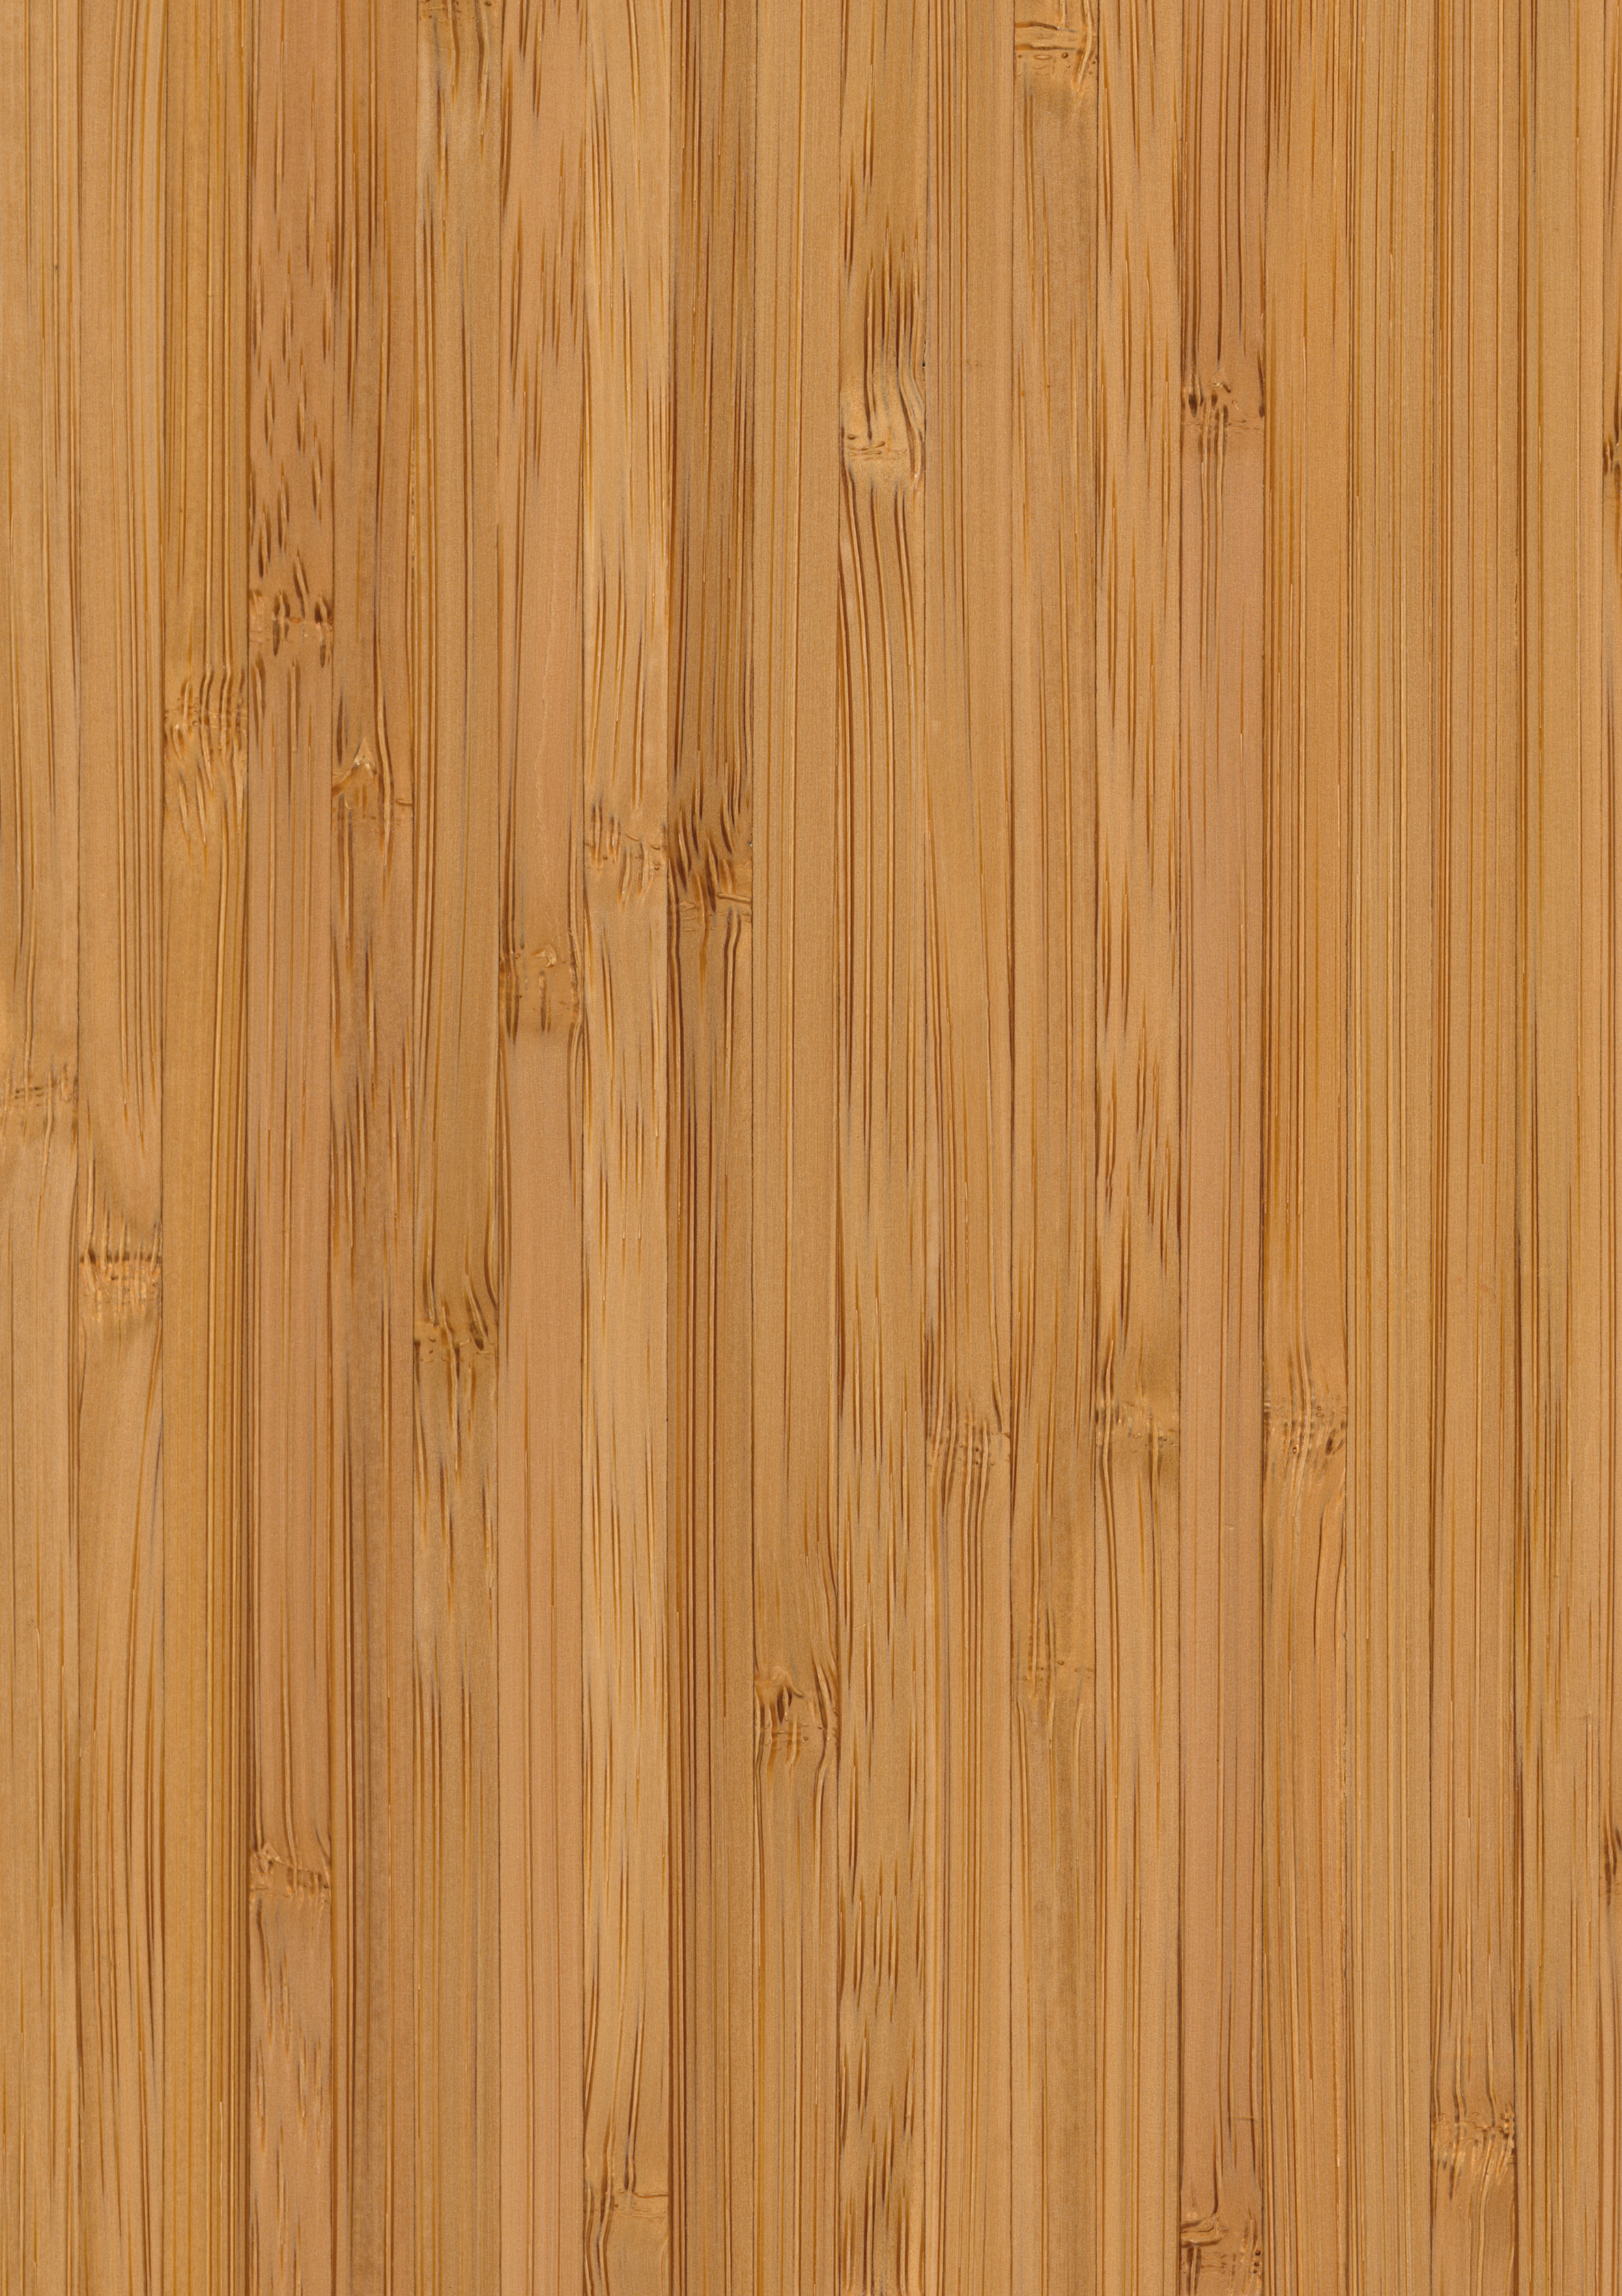
\includegraphics[width=\paperwidth,height=\paperheight]{pictures/bamboo-vert.png}};
    
    \node at ($(bottomleft) + (0.5\paperwidth,2.5cm)$) {
    \fontsize{48}{58}\selectfont
    % these dont want to centre vertically
    \begin{tabular}{rl}
    \multirow{1}{*}{\includegraphics[height=2.5cm]{pictures/vgc_logo_720p.png}}
    &
    \multirow{1}{*}{\rule{0pt}{1.1em}\textrm{\textsc{Victoria Go Club}}} \\
    \end{tabular}
    };
    
    % path fading=north, 
    % \fill[inner sep=0pt, path fading=north, line width=0pt, color=black]%
    % (bottomleft) rectangle (topright);
    
    % % +1cm shouldnt be needed, but apparently the fade makes the fill smaller
    % \fill[inner sep=0pt, path fading=south, line width=0pt, color=VicGreen]%
    % ($(bottomleft)+(0cm, 50cm)$) rectangle ($(topright)+(1cm,1cm)$);
    
    \maketitle

    % >{\raggedright\arraybackslash}
    \begin{columns}
    \column{.025}
    \column{.95}
    \block{\fontsize{35}{40}\selectfont Brief History}{
        \setlength\tabcolsep{1em}
        \begin{center}
        \begin{tabular}{p{.1\textwidth} p{.1\textwidth} p{.1\textwidth} p{.1\textwidth} p{.1\textwidth} p{.1\textwidth} p{.1\textwidth}}
            \includegraphics[width=.1\textwidth]{pictures/Creation.png} & 
            \includegraphics[width=.1\textwidth]{pictures/Monk_Do-rim.png} & 
            \includegraphics[width=.1\textwidth]{pictures/Kibi_no_Makibi.png} & 
            \includegraphics[width=.1\textwidth]{pictures/Honinbou.png} & 
            \includegraphics[width=.1\textwidth]{pictures/Oscar_Korschelt.png} & 
            \includegraphics[width=.1\textwidth]{pictures/Hikaru_no_Go.png} & 
            \includegraphics[width=.1\textwidth]{pictures/AlphaGo.png} \\
            {\sloppy \textbf{??? BC} -  Thousands of years ago the Chinese developed a game called Weiqi, the ``encirclement board game''. } &
            \textbf{475 CE} - The first known mention of Weiqi in Korea, where it is called Baduk. &
            \textbf{715 CE} - Kibi no Makibi introduces Weiqi to Japan, where it is called Igo. &
            \textbf{1612 CE} - Honinbō is founded in Japan. It is the strongest Go school until its closure in 1940. &
            \textbf{1884 CE} - Oscar Korschelt takes Igo from Japan to Europe, where it is called Go. &
            \textbf{1998 CE} - Hikaru no Go, a Japanese manga series, inspires a new generation of Go players. &
            \textbf{2016 CE} - AlphaGo becomes the first computer to win against a top professional.\\
        \end{tabular}
        \end{center}
        
    }
    \column{.025}
    \end{columns}
    

    

    \block{\fontsize{35}{40}\selectfont Basic Rules \vphantom{g}}{
    
        \gobanuse{default}
        \gobanclear
        \gobansize{9}{9}
    
        \gobannew{play}
        \gobanuse{play}
        \gobansize{9}{9}
        \gobanplaceseq{black}{ee, ce, cf, df, de, cg, bf, cd, dc, cc, dg}
        
        \gobannew{capture}
        \gobanuse{capture}
        \gobansize{9}{9}
        \gobanplaceseq[0][\gobanseqnone]{black}{ee, ce, cf, df, de, --, bf, cd, dc, cc, dg, ef, ff, eg, dh, eh, ch, fe, fd, ge, gf, gd, ec, be, bg, fb, fh, db, fg, eb, hf, dd, ei}
        \gobanmark[][cross]{df, ef, eg, eh}
        
        \gobannew{finished}
        \gobanuse{finished}
        \gobansize{9}{9}
        \gobanplaceseq[0][\gobanseqnone]{black}{ee, ce, cf, --, de, --, bf, cd, dc, cc, dg, --, ff, --, dh, --, ch, fe, fd, ge, gf, gd, ec, be, bg, fb, fh, db, fg, eb, hf, dd, ei, ed, hd, he, ie, gc, hc, hb, ib, ha, if, af, ag, ae, id, ia, ic}
        \gobanmark[][cross]{dc, ec, fd}
        \gobanmark[white][square]{aa, ba, ca, da, ea, fa, ga, ab, bb, cb, gb, ac, bc, fc, ad, bd}
        \gobanmark[black][square]{ai, bi, ci, di, fi, gi, hi, ii, ah, bh, eh, gh, hh, ih, cg, eg, gg, hg, ig, df, ef}
    
    
        \vspace{-1em}
        \newcolumntype{Y}{>{\centering\arraybackslash}X}
        \begin{center}
        {\fontsize{25}{30}\selectfont
        \begin{tabularx}{0.9\textwidth}{YYYY}
            \multicolumn{4}{c}{Go is generally played on a 19$\times$19 board, but 13$\times$13 and 9$\times$9 are also used.} \\

            \gobanuse{default} \gobanshowfull[11mm]{} &
            \gobanuse{play} \gobanshowfull[11mm]{} &
            \gobanuse{capture} \gobanshowfull[11mm]{} &
            \gobanuse{finished} \gobanshowfull[11mm]{} \\
            
            {The game starts on an empty board.} &
            {Black and White take turns placing} &
            {Stones are removed from the board} &
            {When the game ends, the player}\\
            
            {Black plays the first move.} &
            {stones on empty intersections.} &
            {when they are completely surrounded.} &
            {with the largest area wins.}\\ % and stones 
        \end{tabularx}
        }
        \end{center}
        \vspace{-14pt}
    }
    
    
    %\begin{columns}
    %\column{.05}
    %\column{.9}
    
    \block{\fontsize{35}{40}\selectfont Capturing Stones}{
    
        \gobansize{9}{9}
    
    
        \gobannew{liberties}
        \gobanuse{liberties}
        \gobansize{9}{9}
        \gobanplace{white}{cc, gi, hi, ii}
        \gobanplace{black}{gd, ge, fe, ai}
        \gobanmark[][triangle]{
            cb, cd, dc, bc,
            gc, hd, he, gf, ff, ee, fd,
            ah, bi,
            fi, gh, hh, ih
        }
        
        
        \gobannew{atari1}
        \gobanuse{atari1}
        \gobansize{9}{9}
        \gobanplace{white}{de, ee, fe}
        \gobanplace{black}{ce, dd, ed, ge, df, ef, ff}
        \gobanmark[][triangle]{fd}
        
        \gobannew{atari2}
        \gobanuse{atari2}
        \gobansize{9}{9}
        \gobanplace[][cross]{white}{de, ee, fe}
        \gobanplace{black}{ce, dd, ed, ge, df, ef, ff, fd[][triangle]}
        
        \gobannew{atari3}
        \gobanuse{atari3}
        \gobansize{9}{9}
        \gobanplace{black}{ce, dd, ed, ge, df, ef, ff, fd[][triangle]}
        
        
        \gobannew{living}
        \gobanuse{living}
        \gobansize{9}{9}
        \gobanplace{white}{
            ad, bd, cd, ce, ae, cf, bf, af,
            ib, hb, gb, fb, fc, fd, fe, ff, fg, fh, gh, hh, ih
        }
        \gobanplace{black}{
            ac, bc, cc, dc, dd, de, df, dg, cg, bg, ag,
            ic, hc, gc, gd, ge, he, gf, gg, hg, ig, id, ie, if
        }
        \gobanmark[][triangle]{be, hd, hf}
        
        
        \newcolumntype{Y}{>{\centering\arraybackslash}X}
        \setlength\tabcolsep{12pt}
        
        \begin{center}
        %\begin{tabular}{p{0.15\textwidth} p{0.15\textwidth} p{0.15\textwidth} p{0.15\textwidth} p{0.15\textwidth}}
        
        \vspace{-2em}
        \begin{tabularx}{1\linewidth}{p{0.2\linewidth}Yp{0.2\linewidth}}
        
        \begin{tabular}{c}
        \rule{0pt}{2em} \\
        \multicolumn{1}{c}
        {\gobanuse{liberties} \gobanshowfull[10mm]{}} \\
        \multicolumn{1}{p{\dimexpr\linewidth-\tabcolsep*2}}
        % Stones of the one color form a group when connected 
        {Stones in a group must be directly adjacent (not diagonally). The liberties \gobantextstone[][triangle]{} of each stone make up the liberties of the group. All groups on the board always have at least one liberty.}
        \end{tabular}
        
        &
        
        \begin{tabular}{p{0.3\linewidth}p{0.3\linewidth}p{0.3\linewidth}}
        
        \multicolumn{3}{c}{\fontsize{25}{30}\selectfont \rule[-0.5em]{0pt}{0pt} Stones of one colour form a group when directly adjacent.} \\
        \multicolumn{3}{c}{\fontsize{25}{30}\selectfont \rule[-0.5em]{0pt}{0pt} Liberties are empty intersections directly adjacent to a group.} \\
        \multicolumn{3}{c}{\fontsize{25}{30}\selectfont \rule[-1em]{0pt}{0pt} Groups are captured when they have no liberties.} \\
        
        \hline
        \rule[-1.5em]{0pt}{0pt} & & \\
        
        \multicolumn{1}{c}
        {\gobanuse{atari1} \gobanshow[10mm]{bc}{hg}} &
        \multicolumn{1}{c}
        {\gobanuse{atari2} \gobanshow[10mm]{bc}{hg}} &
        \multicolumn{1}{c}
        {\gobanuse{atari3} \gobanshow[10mm]{bc}{hg}} \\
        
        \multicolumn{1}{p{0.33\dimexpr\linewidth-\tabcolsep*6}}
        {\rule{0pt}{1.5em}Liberties can be removed by placing stones next to an opposing group.} &
        \multicolumn{1}{p{0.33\dimexpr\linewidth-\tabcolsep*6}}
        {If Black places a stone on the last liberty of the White group, Black captures the group.} &
        \multicolumn{1}{p{0.33\dimexpr\linewidth-\tabcolsep*6}}
        {When captured, all stones in the captured group are removed.} \\
        
        \end{tabular}
        
        &
        
        \begin{tabular}{c}
        \rule{0pt}{2em} \\
        \multicolumn{1}{c}
        {\gobanuse{living} \gobanshowfull[10mm]{}} \\
        \multicolumn{1}{p{\dimexpr\linewidth-\tabcolsep*2}}
        {Surrounding the outside of a group does not always capture it as all liberties must be filled in. A group is safe if it has at least two ``eyes''. White on the left can be captured, but Black on the right cannot.}
        \end{tabular}
        
        \end{tabularx}
        \end{center}
        \vspace{-44pt}
        
        % \begin{tabularx}{1\linewidth}{YYYYY}
        
        % \multicolumn{1}{c|}{} &
        % \multicolumn{3}{c}{\fontsize{25}{30}\selectfont \rule[-0.5em]{0pt}{0pt} Stones of one colour form a group when directly adjacent.} & 
        % \multicolumn{1}{|c}{} \\
        
        % \multicolumn{1}{c|}{} &
        % \multicolumn{3}{c}{\fontsize{25}{30}\selectfont \rule[-0.5em]{0pt}{0pt} Liberties are empty intersections directly adjacent to a group.} & 
        % \multicolumn{1}{|c}{} \\
        
        % \multicolumn{1}{c|}{} &
        % \multicolumn{3}{c}{\fontsize{25}{30}\selectfont \rule[-0.5em]{0pt}{0pt} Groups are captured when they have no liberties.} & 
        % \multicolumn{1}{|c}{} \\ \cline{2-4}
        
        % %\multicolumn{1}{c|}
        % {\gobanuse{liberties} \gobanshowfull[1.5em]{}} &
        % %\multicolumn{1}{c}
        % {\gobanuse{atari1} \gobanshow[1.5em]{bc}{hg}} &
        % %\multicolumn{1}{c}
        % {\gobanuse{atari2} \gobanshow[1.5em]{bc}{hg}} &
        % %\multicolumn{1}{c}
        % {\gobanuse{atari3} \gobanshow[1.5em]{bc}{hg}} &
        % %\multicolumn{1}{|c}
        % {\gobanuse{living} \gobanshowfull[1.5em]{}} \\
        
        % %\multicolumn{1}{p{0.15\textwidth}|}
        % {Stones of the one color form a group when connected directly adjacently (not diagonally). All the liberties of each group stone make up the liberties of the group. All groups on the board must have at least one liberty.} &
        % %\multicolumn{1}{p{0.15\textwidth}}
        % {Liberties can be removed by playing stones next to an opposing group of stones.} &
        % %\multicolumn{1}{p{0.15\textwidth}}
        % {If black places a stone on the last liberty of white, black captures the group of stones.} &
        % %\multicolumn{1}{p{0.15\textwidth}}
        % {When captured, all stones in the captured group are removed from the board.} &
        % %\multicolumn{1}{|p{0.15\textwidth}}
        % {Surrounding the outside of a group does not always capture it as all liberties must be filled in. A group is only ever truly safe if it has at least two "eyes". For example white on the left can be captured, but Black on the right can not.} \\
        
        % \end{tabularx}
        
        
        
        
        
        % \begin{center}
        % \begin{tabular}{p{0.2\textwidth} p{0.1\textwidth} p{0.1\textwidth} p{0.1\textwidth} p{0.2\textwidth}}

        % \multicolumn{1}{c|}{\multirow{2}{*}{liberties diagram}} &
        % \multicolumn{3}{p{0.3\textwidth}}{Stones of one colour form a group when directly adjacent. \newline Liberties are empty intersections directly adjacent to a group. \newline Groups are captured when they have no liberties.} & 
        % \multicolumn{1}{|c}{\multirow{2}{*}{living diagram}} \\ \cline{2-4}
        
        % \multicolumn{1}{p{0.2\textwidth}|}{} &
        % \multicolumn{1}{p{0.1\textwidth}}{atari1 diagram} &
        % \multicolumn{1}{p{0.1\textwidth}}{atari2 diagram} &
        % \multicolumn{1}{p{0.1\textwidth}}{atari3 diagram} &
        % \multicolumn{1}{|p{0.2\textwidth}}{} \\
        
        % \multicolumn{1}{p{0.2\textwidth}|}{descr} &
        % \multicolumn{1}{p{0.1\textwidth}}{descr} &
        % \multicolumn{1}{p{0.1\textwidth}}{descr} &
        % \multicolumn{1}{p{0.1\textwidth}}{descr} &
        % \multicolumn{1}{|p{0.2\textwidth}}{descr} \\
        
        % \end{tabular}
        % \end{center}
        
        % \tabitem Stones of one colour form a group when directly adjacent. \newline \tabitem Liberties are empty intersections directly adjacent to a group. \newline \tabitem Groups are captured when they have no liberties.
        
    }
    
    
    %\column{.05}
    %\end{columns}
    
    
    \begin{columns}
    % \column{.05}
    
    \column{.35}
    \block{\fontsize{35}{40}\selectfont Ko \vphantom{g}}{
        
        \begin{minipage}[l][12cm]{\linewidth}
        
        \gobannew{ko1}
        \gobanuse{ko1}
        \gobansize{9}{9}
        \gobanplace{black}{ed, de, ef}
        \gobanplace{white}{fd, ee, ge, ff}
        
        \gobannew{ko2}
        \gobanuse{ko2}
        \gobansize{9}{9}
        \gobanplace{black}{ed, de, ef, fe}
        \gobanplace{white}{fd, ge, ff}
        \gobanmark[][triangle]{ee}
        
        \setlength\tabcolsep{12pt}
        \newcolumntype{Y}{>{\centering\arraybackslash}X}
        \begin{center}
        \begin{tabularx}{1\linewidth}{YY}
            \multicolumn{2}{c}{\fontsize{25}{30}\selectfont \rule[-1em]{0pt}{0pt} Moves cannot repeat a board state.} \\
            %\multicolumn{1}{c}
            {\gobanuse{ko1} \gobanshowfull[8mm]{}} &
            %\multicolumn{1}{c}
            {\gobanuse{ko2} \gobanshowfull[8mm]{}} \\
            \multicolumn{2}{p{\dimexpr\linewidth-\tabcolsep*2}}{This rule is called Ko. When Black captures the White stone, White cannot immediately capture the Black stone because this could lead to a never ending game. White has to play elsewhere.} \\
        \end{tabularx}
        \end{center}
        
        \end{minipage}
        
    }
    
    
    \column{.65}
    \block{\fontsize{35}{40}\selectfont Ending a Game}{
        
        \begin{minipage}[l][12cm]{\linewidth}
        
        \gobannew{endgame}
        \gobanuse{endgame}
        \gobansize{9}{9}
        \gobanplaceseq[0][\gobanseqnone]{black}{ee, ce, cf, --, de, --, bf, cd, dc, cc, dg, --, ff, --, dh, --, ch, fe, fd, ge, gf, gd, ec, be, bg, fb, fh, db, fg, eb, hf, dd, ei, ed, hd, he, ie, gc, hc, hb, ib, ha, if, af, ag, ae, id, ia, ic}
    
        
        \gobannew{remove}
        \gobanuse{remove}
        \gobansize{9}{9}
        \gobanplaceseq[0][\gobanseqnone]{black}{ee, ce, cf, --, de, --, bf, cd, dc, cc, dg, --, ff, --, dh, --, ch, fe, fd, ge, gf, gd, ec, be, bg, fb, fh, db, fg, eb, hf, dd, ei, ed, hd, he, ie, gc, hc, hb, ib, ha, if, af, ag, ae, id, ia, ic}
        \gobanmark[][cross]{dc, ec, fd}
        
        \gobannew{count}
        \gobanuse{count}
        \gobansize{9}{9}
        \gobanplaceseq[0][\gobanseqnone]{black}{ee, ce, cf, --, de, --, bf, cd, --, cc, dg, --, ff, --, dh, --, ch, fe, --, ge, gf, gd, --, be, bg, fb, fh, db, fg, eb, hf, dd, ei, ed, hd, he, ie, gc, hc, hb, ib, ha, if, af, ag, ae, id, ia, ic}
        % TODO filled square
        \gobanmark[white][square]{aa, ba, ca, da, ea, fa, ga, ab, bb, cb, gb, ac, bc, dc, ec, fc, ad, bd, fd}
        \gobanmark[black][square]{ai, bi, ci, di, fi, gi, hi, ii, ah, bh, eh, gh, hh, ih, cg, eg, gg, hg, ig, df, ef}
        
        \gobannew{closeup}
        \gobanuse{closeup}
        \gobansize{9}{9}
        % @JOSH unless im missing something, 22+21=43
        \gobanplace{black}{de[43]} % 22 stones, 21 territory or 21 territory, 5 captured
        \gobanplace{white}{fe[45]} % 19 stones, 19 territory, 7 komi or 19 territory, 3 captured, 7 komi
    
        \setlength\tabcolsep{12pt}
        \newcolumntype{Y}{>{\centering\arraybackslash}X}
        \begin{center}
        \begin{tabularx}{1\linewidth}{YYYY}
            \multicolumn{2}{c|}{\fontsize{25}{30}\selectfont \rule[-1em]{0pt}{0pt} The game ends when both players pass.} &
            \multicolumn{2}{c}{\fontsize{25}{30}\selectfont \rule[-1em]{0pt}{0pt} The player with the largest area wins.} \\
            \multicolumn{1}{c}{\gobanuse{endgame} \gobanshowfull[8mm]{}} &
            \multicolumn{1}{c|}{\gobanuse{remove} \gobanshowfull[8mm]{}} &
            \multicolumn{1}{c}{\gobanuse{count} \gobanshowfull[8mm]{}} &
            \multicolumn{1}{c}{\gobanuse{closeup} \gobanshow[20mm]{dd}{ff}} \\
            \multicolumn{2}{p{0.5\dimexpr\linewidth-\tabcolsep*4}|}{
            When a player believes they have no meaningful moves to play, they pass. The game ends when both players pass in succession. ``Dead'' stones are agreed upon and captured. If an agreement is not reached, play resumes.} &
            \multicolumn{2}{p{0.5\dimexpr\linewidth-\tabcolsep*4}}{Territory needs to be completely surrounded before it can be scored. The total score for a player is the sum of stones on the board and the territory that they surround. White also receives Komi, additional points for playing second, usually about 7 depending on rule-set.} \\
        \end{tabularx}
        \end{center}
        
        \end{minipage}
    }
    
    
    % \column{.05}
    \end{columns}

\end{document}




\endinput
